%!TEX root = ../main.tex

\section{Introduction}
\label{s:intro}
% \ewu{we really need to emphasize that this is a HARD problem!!}

Poor data quality is a hard and persistent problem.  
It is estimated to cost the US economy more than \$600 billion
per year~\cite{eckerson2002} and erroneous price data in retail databases
alone cost the US consumers \$2.5 billion each year~\cite{Fan2008}. 
Although data
cleaning tools can purge many errors from a dataset before downstream 
applications use the data, datasets can frequently change as applications
and users execute queries that modify the data.
Mistakes in these queries can introduce errors to the data, and these
errors can propagate to more data by subsequent update queries.
By the time errors are detected, their origin has often been obscured and it is difficult to identify the offending query and correct it.
Identifying and correcting errors in the data directly is suboptimal, as it targets the symptom,
rather than the underlying cause. Fixing the manifested data errors on a
case-by-case basis often obscures the root of the problem and other data that may have been
affected. Therefore, traditional data cleaning approaches are not well-suited
for this setting: While they provide general-purpose tools to identify and
rectify anomalies in the data, they are not designed to diagnose the causes of
errors that are rooted in erroneous updates.
Some data cleaning systems try to identify structural sources of
mistakes~\cite{wang2015}, but they are unable to trace the source of
the mistakes to particular faulty queries.

While improving data quality and correcting data errors has been an important
focus for data management research, handling new errors, introduced during
regular database interactions, has received little attention. Most work in
this direction focuses on \emph{guarding against} erroneous updates. For
example, integrity constraints~\cite{Khoussainova2006} reject some improper
updates, 
but only if the data falls outside rigid, predefined ranges.
Certificate-based verification~\cite{Chen2011} is less rigid, but it is
impractical and non-scalable as it requires users to answer challenge
questions before allowing the updates, and it is not applicable to updates
initiated by applications.

\looseness -1
In this paper, we present \sys, a \emph{diagnosis and repair} framework for data errors
caused by erroneous updates. In contrast to existing approaches in data
cleaning that aim to detect and correct errors in the data directly, the goal
of \sys is to identify errors in the queries that introduced errors in the
data. These diagnoses \emph{explain} how errors were introduced to a
dataset, and allow an administrator to easily identify and further validate the most likely query-based sources of these errors. 
In addition, once the erroneous queries have been confirmed, repairing the source of the errors
can potentially lead to the identification of additional discrepancies in
the data that would have otherwise remained undetected.  
We describe two motivating examples; the first is a real-life scenario, provided to us by a large US-based wireless provider.
% 
\begin{example}[Wireless discount policies]\label{ex:telco}

A wireless provider offers company discounts as incentives for
corporate customers. There are different types of discounts (flat, percentage,
fee-based), and their details are specific to corporate agreements. The large
number of policies and complexities in their rules frequently cause policies
to be set incorrectly, leading to errors in the application of discounts to
customers' accounts.

\looseness -1
Customers who notice billing errors contact the provider, but the call centers
do not have the capacity or ability to investigate the complaints deeply. The
standard course of action is to correct mistakes on a case-by-case
basis for each complaint. As a result, unreported errors remain in the
database for a long time, or they never get corrected, and their cause becomes
harder to trace as further queries modify the database.%  the source of the errors is obscured.
% \footnote{This is a real-life scenario, provided to us by a large US-based wireless provider.}

\end{example}
% 
\begin{example}[Tax bracket adjustment]\label{ex:taxes}
    
Tax brackets determine tax rates for different income levels and are
often adjusted. Accounting firms implement these changes to their
databases by appropriately updating the tax rates of their customers. Mistakes
in these update queries (e.g., Figure~\ref{fig:example}) result in errors in
the tax rates and computed taxes. 

\end{example}
% 
In these application scenarios, data errors are typically reported to
a customer service department, which does not have the resources nor
the capability to investigate the errors more broadly. Instead, errors
are resolved on a case-by-case basis. The goal of \sys is to identify
the query or queries that caused the errors and propose corrections to
those queries.  Once these repairs have been validated (say, by an expert), they can be used to identify unreported
errors and to prevent the introduction of more errors. This problem
has the following important characteristics that render it very difficult, and unsuitable for traditional
techniques:


\begin{description}[leftmargin=*, topsep=0mm, itemsep=0mm]
    
    \item[Obscurity.] \looseness -1
    % Detection of the resulting errors in the data often
    Handling data errors directly often
    leads to partial fixes that further complicate the eventual diagnosis and
    resolution of the problem. For example, a transaction implementing a
    change in the state tax law updated tax rates using the wrong rate,
    affecting a large number of consumers. This causes a large number of
    complaints to a call center, but each customer agent usually fixes each
    problem individually, which ends up obscuring the source of the problem.
    
    \item[Large impact.] Erroneous queries cause errors at a large scale. The
    potential impact of the errors is high, as manifested in several
    real-world cases~\cite{Yates10, Grady13, sakalerrors}. Further, errors
    that remain undetected for a significant amount of time can instigate
    additional errors, even through valid updates. This increases both their
    impact, and their obscurity.
    
    \item[Systemic errors.] The errors created by bad queries are
    \emph{systemic}: they have common characteristics, as they share the same
    cause. The link between the resulting data errors is the query that
    created them; cleaning techniques should leverage this connection to
    diagnose and fix the problem. Diagnosing the cause of the errors, will
    achieve systematic fixes that will correct all relevant errors, even if
    they have not been explicitly identified.
    
\end{description}
% 
\sys does not replace traditional data cleaning methods, but rather, complements them.
Instead of identifying errors in the data directly, 
\sys targets the diagnosis, explanation, and repair of errors at the root by
leveraging example errors acquired from 
users, traditional data cleaning, or detection techniques.

Diagnosing data errors stemming from incorrect updates is fundamentally
challenging: the search space of possible mistakes and fixes is large, and the
amount of information (number of known errors) may be limited. 
\sys addresses these challenges by analyzing the queries that operated on a
dataset in an efficient and scalable manner. More concretely, we make the
following contributions:


% The goal of this paper is to design effective query
% diagnosis techniques and identify possible fixes for query errors. We
% model the problem assuming a log of update workloads over a database,
% and a set of complaints that identify errors in the final database
% state. We organize our contributions as follows:

% \ewu{really like this organization}

% \ewu{add: special case optimizations for single query case.}

\begin{itemize}[leftmargin=*, topsep=0mm, itemsep=0mm]      
    \item We formalize the problem of diagnosing a set of errors using log
    histories of updates that operated on the data. Given a set of 
    \emph{complaints} as representations of data discrepancies in the current
    state of a dataset, \sys determines how to resolve all of the complaints with the minimal amount of changes to the queries in the log (Section~\ref{sec:abstractions}).
    % identifies the queries in the log that require the  minimal
    % amount of changes (to the original query log) 
    % that would resolve all of the complaints (Section~\ref{sec:abstractions}).
      
    \item We provide an exact error-diagnosis solution through a non-trivial
    transformation of the problem to a mixed integer linear program (MILP) that
    encodes the data provenance of the erroneous tuples. Our approach employs state-of-the-art MILP solvers to identify
    optimal diagnoses that are guaranteed to resolve all complaints without introducing new errors to the data
    (Section~\ref{sec:sol}).
    
    \item We present several optimizations to our basic diagnostic
    method, which reduce the problem size without affecting the
    quality of the produced solutions. Further, we propose an
    incremental repair method that targets the cases where the log
    contains a single corrupted query (or the search focuses on a
    single repair). This incremental analysis of the log allows us to
    scale to large datasets ($100k$ records) and large query logs (hundreds to thousands of update queries). Further, we
    show that our optimization techniques have the additional
    advantage of tolerating incomplete information, such as unreported
    errors (Section~\ref{sec:opt}). 

    
    % \item We extend our framework to also handle false positives: complaints
    % that mistakenly identify data as erroneous. We define the notion of
    % complaint \emph{density}, which is a query-driven measure of closeness of
    % a complaint to other complaints. The main intuition of our approach is
    % that complaints of low density are likely false positives and thus can be
    % safely ignored (Section~\ref{???}).
    
    \item We perform a thorough evaluation of the trade-offs between speed and accuracy of our baseline and optimized methods under a controlled, synthetic setting. In particular, we demonstrate that the  \sys optimizations achieve significant speedup compared to the baseline algorithm (40$\times$ in some of our experimental settings).
    We also evaluate \sys on common OLTP benchmarks and show how \sys can propose fully accurate repairs within milliseconds on a TPC-C workload with $1500$ queries (Section~\ref{sec:experiments}).
    %experimentally evaluate the effectiveness and efficiency of our
    %methods against benchmark and synthetic datasets and query logs. 
\end{itemize}

To the best of our knowledge, \sys is the first system that diagnoses
and repairs errors through query histories. We show that it is
extremely effective and efficient with the update workloads found in
most common benchmarks. 
While \sys trusts its input to be correct, it
can handle incomplete information, and it can be resilient to some
inaccuracies in the reported data errors (Section~\ref{sec:noise}).
\sys does not handle some complex query types
that are less common in update workloads, such as nested queries,
joins, and aggregation. 
It also does not currently deal with large amounts of incorrect
information, such as fake data errors reported by malicious users.
These challenges present exciting future extensions to the system presented in this work.
% this challenge is orthogonal to the goals of \sys and to the focus of our work.






\section{{\large\textbf{\sys}}: architecture}




Figure~\ref{fig:architecture} shows the architecture of \sys. The system uses
two inputs: a log of update queries (including UPDATE, INSERT, and DELETE
statements) and a set of identified data errors (\emph{complaints}). \sys
analyzes the data errors and the query logs to trace the causes of the errors
in queries in the log (diagnoses), and to automatically derive query repairs.
The query repairs represent corrections to the queries in the log, and can be
used to identify additional errors in the data that were not reported.
% 
The core of \sys is a transformation module that expresses the query diagnosis
problem as a Mixed Integer Linear Program (MILP). Two performance optimization modules
ensure that the system can scale to large datasets efficiently, while
maintaining high accuracy. 
% Finally, the density filtering component ensures
% smooth handling of false errors (data that has been identified as erroneous,
% but it is in fact correct).

% \alex{Xiaolan, please add a couple of sentences on implementation.}

\begin{figure}[t]
    \centering
        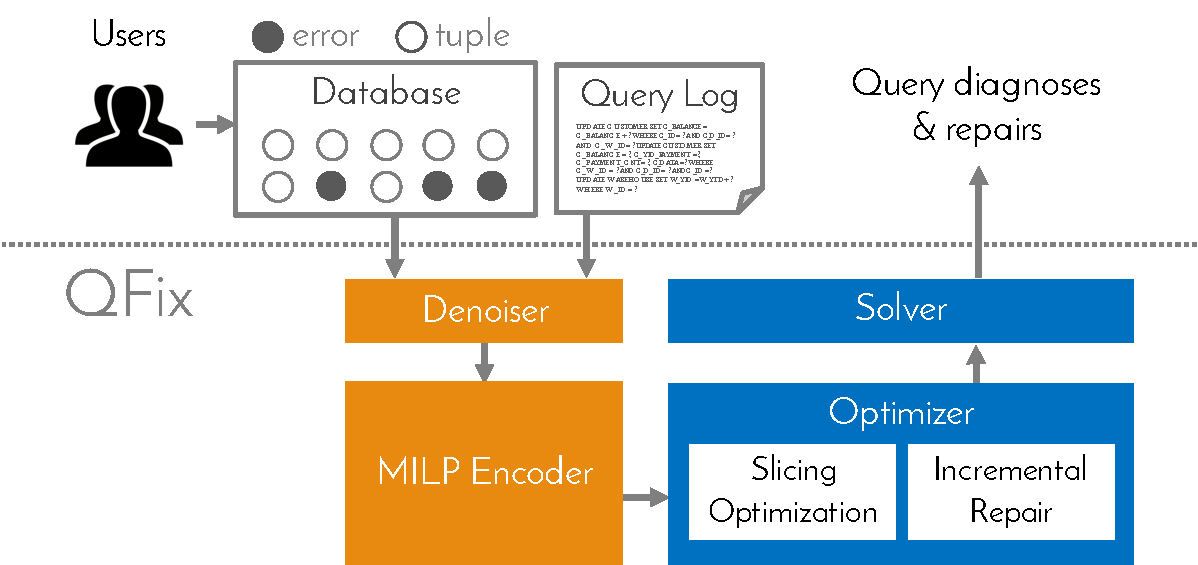
\includegraphics[scale=0.35]{figures/architecture}
    \caption{\sys processes data anomalies in the form of complaints and analyzes logged query histories to identify the causes of error. In the heart of the system, transformation algorithms express the diagnosis problem as a mixed integer linear program (MILP), and optimization modules ensure that the MILP programs can be evaluated efficiently.}
\vspace*{-0.1in}
    \label{fig:architecture}
\end{figure}

